\documentclass[a4paper,12pt]{article}
\usepackage[utf8]{inputenc}
\usepackage[T1]{fontenc}
\usepackage[english]{babel}
\usepackage{lmodern}
\usepackage{amsmath}
\usepackage{amssymb}
\usepackage{amsthm}
\usepackage[superscript]{cite}
\usepackage{nicefrac}
\usepackage{upgreek}
\usepackage{paralist}
\usepackage{stmaryrd}
\usepackage{tikz}
\usepackage{graphicx}
\usepackage{qtree}
\usepackage{dsfont}
\usepackage{eurosym}
\usepackage{tabulary}
\usepackage{setspace}
\usepackage{fancyhdr}
% \usepackage[colorlinks=true,linkcolor=blue]{hyperref}				% Blaue Links sehen meiner Ansicht nach besser aus als die rot umrandeten Verweise

% Kopfzeile
\newcommand\shorttitle{ROI Hypothesis Testing}
\newcommand\authors{Dominik Blank}

\fancyhf{} % sets all head and foot elements empty
\fancyhead[L]{\shorttitle}
\fancyhead[R]{\authors}
\pagestyle{fancy} % sets the page style to the style delivered and editable with fancyhdr

% Kommandos, Operatoren, etc.
\newcommand{\abs}[1]{\lvert#1\rvert}
\newcommand{\norm}[1]{\lVert#1\rVert}
\DeclareMathOperator{\thetafunc}{\uptheta}

% Mathe-Umgebungen
\theoremstyle{plain}
\newtheorem{theorem}{Theorem}
\newtheorem{lemma}{Lemma}
\newtheorem{corollary}{Corollary}
\theoremstyle{definition}
\newtheorem{definition}{Definition}
\theoremstyle{remark}
\newtheorem{remark}{Remark}
\newtheorem{example}{Example}

% ENDE PRÄAMBEL

\author{Dominik Blank}
\title{Gleichmäßige obere Schranken beim Kreisproblem}

\onehalfspacing
\setlength{\parindent}{0pt}
\allowdisplaybreaks

\begin{document}
%\begin{titlepage}
%
%\newcommand{\HRule}{\rule{\linewidth}{0.5mm}} % Defines a new command for the horizontal lines, change thickness here
%
%\center % Center everything on the page
% 
%%----------------------------------------------------------------------------------------
%%	HEADING SECTIONS
%%----------------------------------------------------------------------------------------
%
%\textsc{\Large Georg-August-Universität Göttingen}\\[1.5cm] % Name of your university/college
%\textsc{\large Bachelor-Arbeit zum Thema}\\[0.5cm] % Major heading such as course name
%% \textsc{\large Minor Heading}\\[0.5cm] % Minor heading such as course title
%
%%----------------------------------------------------------------------------------------
%%	TITLE SECTION
%%----------------------------------------------------------------------------------------
%
%\HRule \\[0.4cm]
%{\large \bfseries Gleichmäßige obere Schranken beim Kreisproblem}\\[0.2cm] % Title of your document
%\HRule \\[1.5cm]
% 
%%----------------------------------------------------------------------------------------
%%	AUTHOR SECTION
%%----------------------------------------------------------------------------------------
%
%\begin{minipage}{0.4\textwidth}
%\begin{flushleft} \large
%\emph{Autor:}\\
%Dominik \textsc{Blank} % Your name
%\end{flushleft}
%\end{minipage}
%~
%\begin{minipage}{0.5\textwidth}
%\begin{flushright} \large
%\emph{Betreuer:} \\
%Prof. Dr. Valentin \textsc{Blomer} % Supervisor's Name
%\end{flushright}
%\end{minipage}\\[4cm]
%
%%----------------------------------------------------------------------------------------
%%	DATE SECTION
%%----------------------------------------------------------------------------------------
%
%{\large Göttingen, den \today}\\[3cm] % Date, change the \today to a set date if you want to be precise
%
%\begin{abstract}
%	In dieser Arbeit wird eine asymptotische Formel für die ganzzahligen Darstellungen der natürlichen Zahlen $m \leq R$ durch eine positiv-definite quadratische Form hergeleitet.
%	Die implizite Konstante des Fehlerterms wird dabei nicht von der jeweiligen quadratischen Form abhängen.
%\end{abstract}
%\end{titlepage}
%
%\newpage

\tableofcontents

\newpage

\section{ROI Testing}

\subsection{The statistical model}

Let $M, N \in \mathbb{N}$ and $G = \left\{ 0, \dots, M-1 \right\} \times  \left\{ 0, \dots, N-1 \right\}$. Assume we are given data
\begin{equation}\label{f}
	f(i, j) = c_{bg} + v(i, j) + \varepsilon_{i, j}
\end{equation}
where $(i, j) \in G$, $c_{bg} \in \mathbb{R}$ is constant, $v: G \to \{ 0, \pm c_{bg} \}$ and $\varepsilon_{i, j} \sim \mathcal{N}(0, \sigma^2)$ are i.i.d. normal distributed random variables for some $\sigma > 0$ and for all $(i, j) \in G$.

We treat $v$ as an image, that contains a rectangular, thus convex, region of interest. That means, that the pixels with value $\pm c_{bg}$ are arranged in a rectangular shape and all other pixels have value $0$.

\subsection{Testing for the ROI}

\subsubsection{Preparations}

For each pair $(i, j) \in G$ we define four values
\begin{align}
	\tilde{d}^\pm_1(i, j) &= f(i \pm 1, j) - f(i, j) \label{d1} \\
	\tilde{d}^\pm_2(i, j) &= f(i, j \pm 1) - f(i, j) \label{d2}
\end{align}
where we define
\begin{align*}
	f(i, -1) &= f(i, N-1) \\
	f(-1, j) &= f(M-1, j) \\
	f(i, N) &= f(i, 0) \\
	f(M, j) &= f(0, j)
\end{align*}
to adjust to boundary issues. We now combine these values into two new values and assign to each pair $(i, j) \in G$ the values
\begin{equation}\label{d_tilde}
	\tilde{d}^\pm(i, j) = \sqrt{\tilde{d}_1^\pm(i, j)^2 + \tilde{d}_2^\pm(i, j)^2}
\end{equation}

We now want to test if a pixel is part of the aforementioned region of interest (ROI). To do this, we define another two values for each pixel $(i, j) \in G$:
\begin{equation}\label{d}
	d^\pm(i, j) = \sqrt{(v(i \pm 1, j) - v(i, j))^2 + (v(i, j \pm 1) - v(i, j))^2}
\end{equation}
Although the definitions of $d^\pm(i, j)$ and $\tilde{d}^\pm(i, j)$ are quite similar, note, that we can only actually compute the values of the latter. The definition of $d^\pm(i, j)$ helps us define a null hypothesis for our testing procedure. Since we want to test for the ROI, our null hypothesis for a given pixel is, that it is a background pixel. That translates to $v(i, j) = 0$. If a pixel is background and since we assumed the ROI to be rectangular, that means, that its top and left neighbour pixels or bottom and right neighbour pixels are background as well. This leads to the null hypothesis
\begin{equation}
	H_0 : \min\{ d^+(i, j), d^-(i, j) \} = 0
\end{equation}
Since by definition $d^\pm(i, j) \geq 0$, our alternative hypothesis becomes
\begin{equation}
	H_1 : \min\{ d^+(i, j), d^-(i, j) \} > 0
\end{equation}

Since $v$ only takes values in $\{ 0, -c_{bg}, c_{bg} \}$, $d^\pm$ also can only attain values in
\begin{equation*}
	\mathcal{D} = \{ 0, c_{bg}, 2 c_{bg}, \sqrt{2} c_{bg}, \sqrt{5} c_{bg}, \sqrt{8} c_{bg} \}
\end{equation*}
This means, that we can define two sets $\mathcal{D}_0$ and $\mathcal{D}_1$ as follows
\begin{equation*}
	\mathcal{D}_1 = ( \mathcal{D} \setminus \{ 0 \} ) \times ( \mathcal{D} \setminus \{ 0 \} )
\end{equation*}
\begin{equation*}
	\mathcal{D}_0 = ( \mathcal{D} \setminus \{ 0 \} ) \times \{ 0 \} \cup \{ 0 \} \times ( \mathcal{D} \setminus \{ 0 \} ) \cup ( \{ 0 \} \times \{ 0 \} ) = ( \mathcal{D} \times \mathcal{D} ) \setminus \mathcal{D}_1
\end{equation*}
Now, if $(d^+, d^-) \in \mathcal{D}_0$ then the null hypothesis is true and if $(d^+, d^-) \in \mathcal{D}_1$, the alternative hypothesis is true.

\subsubsection{Distribution of $\mathbb{P}(\tilde{d}^\pm(i, j) \leq t \mid d^\pm(i, j) = d)$}

We want to determine the distribution of $\tilde{d}^\pm(i, j)$ conditioned on $d^\pm(i, j) = d$ for some $d \in \mathcal{D}$. We define
\begin{align*}
	d_1^\pm(i, j) &= v(i \pm 1, j) - v(i, j) \\
	d_2^\pm(i, j) &= v(i, j \pm 1) - v(i, j)
\end{align*}
Then $d^\pm(i, j) = \sqrt{d_1^\pm(i, j)^2 + d_2^\pm(i, j)^2}$. We note that the roles of $d_1^\pm(i, j)$ and $d_2^\pm(i, j)$ are symmetrical. Furthermore we can see, that for $d^\pm(i, j) = d$ given, we can determine, what $d_1^\pm(i, j)$ and $d_2^\pm(i, j)$ are.

\begin{center}
	\begin{tabular}{c|c|c|c}
		$d$ & $d_1^\pm$ & $d_2^\pm$ & Description \\
		\hline
		$0$ & $0$ & $0$ & Background \\
		\hline
		$c_{bg}$ & $\{ c_{bg}, 0 \}$ & $\{ 0, c_{bg} \}$ & Going from background to foreground \\
		\hline
		$2 c_{bg}$ & $\{ 2 c_{bg}, 0 \}$ & $\{ 0, 2 c_{bg} \}$ & Only theoretical \\
		\hline
		$\sqrt{2} c_{bg}$ & $c_{bg}$ & $c_{bg}$ & Only theoretical \\
		\hline
		$\sqrt{5} c_{bg}$ & $\{ 2 c_{bg}, c_{bg} \}$ & $\{ c_{bg}, 2 c_{bg} \}$ & Going from foreground to background \\
		\hline
		$\sqrt{8} c_{bg}$ & $2 c_{bg}$ & $2 c_{bg}$ & Foreground \\
	\end{tabular}
\end{center}

Using this relation, we get
\begin{align*}
	&\mathbb{P}(\tilde{d}^\pm(i, j) \leq t \mid d^\pm(i, j) = d) \\
	&= \mathbb{P}(( (c_{bg} + v(i \pm 1, j) + \varepsilon_{i \pm 1, j} - c_{bg} - v(i, j) - \varepsilon_{i, j})^2 \\
	&+ (c_{bg} + v(i, j \pm 1) + \varepsilon_{i, j \pm 1} - c_{bg} - v(i, j) - \varepsilon_{i, j})^2 )^{\frac{1}{2}} \leq t \mid d^\pm(i, j) = d) \\
	&= \mathbb{P}\left( \sqrt{(d_1^\pm(i, j) + \varepsilon_{i \pm 1, j} - \varepsilon_{i, j})^2 + (d_2^\pm(i, j) + \varepsilon_{i, j \pm 1} - \varepsilon_{i, j})^2} \leq t \right) \\
	&= \mathbb{P}\left( \sqrt{2} \sigma \sqrt{\left( \frac{X_1}{\sqrt{2} \sigma} \right)^2 + \left( \frac{X_2}{\sqrt{2} \sigma} \right)^2} \leq t \right)
\end{align*}
with
\begin{align*}
	X_1 &= d_1^\pm(i, j) + \varepsilon_{i \pm 1, j} - \varepsilon_{i, j} \sim \mathcal{N}(d_1^\pm(i, j), 2 \sigma^2) \\
	X_2 &= d_2^\pm(i, j) + \varepsilon_{i, j \pm 1} - \varepsilon_{i, j} \sim \mathcal{N}(d_2^\pm(i, j), 2 \sigma^2)
\end{align*}

Then we can see, that the square root inside has non-central chi distribution with two degrees of freedom and parameter
\begin{equation*}
	\lambda = \sqrt{\left( \frac{d_1^\pm}{\sqrt{2} \sigma} \right)^2 + \left( \frac{d_2^\pm}{\sqrt{2} \sigma} \right)^2} = \frac{\sqrt{d_1^\pm(i, j)^2 + d_2^\pm(i, j)^2}}{\sqrt{2} \sigma} = \frac{d^\pm(i, j)}{\sqrt{2} \sigma}
\end{equation*}

The cumulative distribution function of the non-central chi distribution with parameter $\lambda$ and two degrees of freedom is $1 - Q_1(\lambda, x)$, where $Q_M(a, b)$ denotes the Marcum $Q$-function, which is defined as
\begin{equation*}
	Q_M(a, b) = \int_b^\infty x \left( \frac{x}{a} \right)^{M-1} \exp \left( - \frac{x^2 + a^2}{2} \right) I_{M-1}(ax) dx
\end{equation*}
with modified Bessel function $I_{M-1}$.

Putting this together, we obtain
\begin{align*}
	\mathbb{P}(\tilde{d}^\pm(i, j) \leq t \mid d^\pm(i, j) = d) &= \mathbb{P}\left( \sqrt{2} \sigma \sqrt{\left( \frac{X_1}{\sqrt{2} \sigma} \right)^2 + \left( \frac{X_2}{\sqrt{2} \sigma} \right)^2} \leq t \right) \\
	&= \mathbb{P}\left( \sqrt{\left( \frac{X_1}{\sqrt{2} \sigma} \right)^2 + \left( \frac{X_2}{\sqrt{2} \sigma} \right)^2} \leq \frac{t}{\sqrt{2} \sigma} \right) \\
	&= 1 - Q_1 \left( \frac{d}{\sqrt{2} \sigma}, \frac{t}{\sqrt{2} \sigma} \right)
\end{align*}

For $d = 0$ this simplifies a lot and we get
\begin{align*}
	\mathbb{P}(\tilde{d}^\pm(i, j) \leq t \mid d^\pm(i, j) = 0) &= 1 - Q_1 \left( 0, \frac{t}{\sqrt{2} \sigma} \right) \\
	&= 1 - \exp \left( - \frac{t^2}{4 \sigma^2} \right)
\end{align*}

\newpage

For $\mathrm{Re} \ \nu > -1$, $\mathrm{Re} \ \alpha > 0$ we have
\begin{equation*}
	\int_0^\infty \exp \left( - \alpha x^2 \right) I_\nu ( \beta x ) dx = \frac{\sqrt{\pi}}{2 \sqrt{\alpha}} \exp \left( \frac{\beta^2}{8 \alpha} \right) I_{\frac{1}{2} \nu} \left( \frac{\beta^2}{8 \alpha} \right)
\end{equation*}

For $p \neq b$ and $s = \sqrt{p^2 - b^2}$, $u = \sqrt{a (p - s)}$ and $v = \sqrt{a (p + s)}$ we have
\begin{equation*}
	\int_0^a \exp(-p x) I_M ( b x ) dx = \frac{1}{s b^M} \left( (p - s)^M ( 1 - Q_M(u, v) ) - (p + s)^M ( 1 - Q_M(v, u) ) \right)
\end{equation*}

Note, that the Marcum $Q$-Function is only defined for $M \geq 1$. For $M = 1$ this simplifies to
\begin{equation*}
	\int_0^a \exp(-p x) I_1 ( b x ) dx = \frac{1}{s b} \left( (p - s) ( 1 - Q_1(u, v) ) - (p + s) ( 1 - Q_1(v, u) ) \right)
\end{equation*}

We get for fixed $\varepsilon_{i, j}$:
\begin{align*}
	&\mathbb{P}(\tilde{d}^\pm(i, j) \leq t \mid d^\pm(i, j) = d) \\
	&= \mathbb{P}( (c_{bg} + v(i \pm 1, j) + \varepsilon_{i \pm 1, j} - c_{bg} - v(i, j) - \varepsilon_{i, j})^2 \\
	&+ (c_{bg} + v(i, j \pm 1) + \varepsilon_{i, j \pm 1} - c_{bg} - v(i, j) - \varepsilon_{i, j})^2 \leq t^2 \mid d^\pm(i, j) = d) \\
	&= \mathbb{P}\left( (d_1^\pm(i, j) + \varepsilon_{i \pm 1, j} - \varepsilon_{i, j})^2 + (d_2^\pm(i, j) + \varepsilon_{i, j \pm 1} - \varepsilon_{i, j})^2 \leq t^2 \right) \\
	&= \mathbb{P}\left( \sqrt{\left( \frac{X_1}{\sigma} \right)^2 + \left( \frac{X_2}{\sigma} \right)^2} \leq \frac{t}{\sigma} \right)
\end{align*}
with
\begin{align*}
	X_1 &= d_1^\pm(i, j) + \varepsilon_{i \pm 1, j} - \varepsilon_{i, j} \sim \mathcal{N}(d_1^\pm(i, j) - \varepsilon_{i, j}, \sigma^2) \\
	X_2 &= d_2^\pm(i, j) + \varepsilon_{i, j \pm 1} - \varepsilon_{i, j} \sim \mathcal{N}(d_2^\pm(i, j) - \varepsilon_{i, j}, \sigma^2)
\end{align*}

Then we can see, that the square root inside has non-central chi distribution with two degrees of freedom and non-centrality parameter
\begin{equation*}
	\lambda = \sqrt{\left( \frac{d_1^\pm - \varepsilon_{i, j}}{\sigma} \right)^2 + \left( \frac{d_2^\pm - \varepsilon_{i, j}}{\sigma} \right)^2} = \frac{\sqrt{(d_1^\pm(i, j) - \varepsilon_{i, j})^2 + (d_2^\pm(i, j) - \varepsilon_{i, j})^2}}{\sigma}
\end{equation*}

For $d^\pm = 0$ this becomes $\lambda = \frac{\sqrt{2} \abs{\varepsilon_{i, j}}}{\sigma}$ and thus we get
\begin{equation*}
	\sqrt{\left( \frac{X_1}{\sigma} \right)^2 + \left( \frac{X_2}{\sigma} \right)^2} \sim \chi_2 \left( \frac{\sqrt{2} \abs{\varepsilon_{i, j}}}{\sigma} \right)
\end{equation*}

So far we assumed $\varepsilon_{i, j}$ to be fixed, but it actually is a random variable itself with normal distribution: $\varepsilon_{i, j} \sim \mathcal{N}(0, \sigma^2)$. Thus, we have a compound probability distribution:
\begin{align*}
	&\mathbb{P}(\tilde{d}^\pm(i, j) \leq t \mid d^\pm(i, j) = 0) \\
	&= \mathbb{P}\left( \sqrt{\left( \frac{X_1}{\sigma} \right)^2 + \left( \frac{X_2}{\sigma} \right)^2} \leq \frac{t}{\sigma} \right) \\
	&= \int_0^\frac{t}{\sigma} \int_0^\infty \underbrace{x \exp \left( - \frac{x^2}{2} - \frac{\eta^2}{\sigma^2} \right) I_0 \left( \frac{\sqrt{2} \eta}{\sigma} x \right)}_{\textrm{pdf of} \ \chi_2 \left( \frac{\sqrt{2} \eta}{\sigma} \right) \ \textrm{for fixed} \ \eta} \underbrace{\frac{2}{\sqrt{2 \pi \sigma^2}} \exp \left( - \frac{\eta^2}{2 \sigma^2} \right)}_{\textrm{pdf of absolute value of} \ \mathcal{N}(0, \sigma^2)} d\eta dx \\
	&= \frac{2}{\sqrt{2 \pi \sigma^2}} \int_0^\frac{t}{\sigma} x \exp \left( - \frac{x^2}{2} \right) \int_0^\infty \exp \left( - \frac{3}{2 \sigma^2} \eta^2 \right) I_0 \left( \frac{\sqrt{2} x}{\sigma} \eta \right) d\eta dx \\
	&= \frac{2}{\sqrt{2 \pi \sigma^2}} \int_0^\frac{t}{\sigma} x \exp \left( - \frac{x^2}{2} \right) \frac{\sqrt{\pi}}{2 \sqrt{\frac{3}{2 \sigma^2}}} \exp \left( \frac{\frac{2 x^2}{\sigma^2}}{8 \frac{3}{2 \sigma^2}} \right) I_0 \left( \frac{\frac{2 x^2}{\sigma^2}}{8 \frac{3}{2 \sigma^2}} \right) dx \\
	&= \frac{1}{\sqrt{3}} \int_0^\frac{t}{\sigma} x \exp \left( - \frac{x^2}{2} \right) \exp \left( \frac{x^2}{6} \right) I_0 \left( \frac{x^2}{6} \right) dx \\
	&= \frac{1}{\sqrt{3}} \int_0^\frac{t}{\sigma} x \exp \left( - \frac{x^2}{3} \right) I_0 \left( \frac{x^2}{6} \right) dx \\
	&= \frac{1}{\sqrt{3}} \left[ - \frac{3}{2} \exp \left( - \frac{x^2}{3} \right) I_0 \left( \frac{x^2}{6} \right) \right]_0^\frac{t}{\sigma} + \frac{1}{2 \sqrt{3}} \int_0^\frac{t}{\sigma} \exp \left( - \frac{x^2}{3} \right) x I_1 \left( \frac{x^2}{6} \right) dx \\
	&= \frac{1}{\sqrt{3}} \left( \frac{3}{2} - \frac{3}{2} \exp \left( - \frac{\left( \frac{t}{\sigma} \right)^2}{3} \right) I_0 \left( \frac{\left( \frac{t}{\sigma} \right)^2}{6} \right) \right) + \frac{1}{2 \sqrt{3}} \int_0^\frac{t}{\sigma} \exp \left( - \frac{x^2}{3} \right) x I_1 \left( \frac{x^2}{6} \right) dx \\
	&\overset{y = x^2}{=} \frac{1}{\sqrt{3}} \left( \frac{3}{2} - \frac{3}{2} \exp \left( - \frac{t^2}{3 \sigma^2} \right) I_0 \left( \frac{t^2}{6 \sigma^2} \right) \right) + \frac{1}{4 \sqrt{3}} \int_0^\frac{t}{\sigma} \exp \left( - \frac{y}{3} \right) I_1 \left( \frac{y}{6} \right) dy \\
	&= \frac{1}{\sqrt{3}} \left( \frac{3}{2} - \frac{3}{2} \exp \left( - \frac{t^2}{3 \sigma^2} \right) I_0 \left( \frac{t^2}{6 \sigma^2} \right) \right) + \frac{1}{4 \sqrt{3}} \int_0^\frac{t}{\sigma} \exp \left( - \frac{y}{3} \right) I_1 \left( \frac{y}{6} \right) dy \\
	&= \frac{1}{\sqrt{3}} \left( \frac{3}{2} - \frac{3}{2} \exp \left( - \frac{t^2}{3 \sigma^2} \right) I_0 \left( \frac{t^2}{6 \sigma^2} \right) \right) \\
	&+ \frac{1}{4 \sqrt{3}} \frac{1}{\frac{1}{2 \sqrt{3}} \frac{1}{6}} \frac{2 - \sqrt{3}}{6} \left( 1 - Q_1 \left( \frac{2 - \sqrt{3}}{6} \sqrt{\frac{t}{\sigma}}, \frac{2 + \sqrt{3}}{6} \sqrt{\frac{t}{\sigma}} \right) \right) \\
	&- \frac{1}{4 \sqrt{3}} \frac{1}{\frac{1}{2 \sqrt{3}} \frac{1}{6}} \frac{2 + \sqrt{3}}{6} \left( 1 - Q_1 \left( \frac{2 + \sqrt{3}}{6} \sqrt{\frac{t}{\sigma}}, \frac{2 - \sqrt{3}}{6} \sqrt{\frac{t}{\sigma}} \right) \right) \\
	&= \frac{1}{\sqrt{3}} \left( \frac{3}{2} - \frac{3}{2} \exp \left( - \frac{t^2}{3 \sigma^2} \right) I_0 \left( \frac{t^2}{6 \sigma^2} \right) \right) - \sqrt{3} \\
	&- \frac{2 - \sqrt{3}}{2} Q_1 \left( \frac{2 - \sqrt{3}}{6} \sqrt{\frac{t}{\sigma}}, \frac{2 + \sqrt{3}}{6} \sqrt{\frac{t}{\sigma}} \right) \\
	&+ \frac{2 + \sqrt{3}}{2} Q_1 \left( \frac{2 + \sqrt{3}}{6} \sqrt{\frac{t}{\sigma}}, \frac{2 - \sqrt{3}}{6} \sqrt{\frac{t}{\sigma}} \right)
\end{align*}

\newpage

\subsubsection{Statistical significance}

We aim to use the law of total probability in the following way. Let $B_n$ be a partition of $B$, that is a countable number of sets, such that $\bigcup_n B_n = B$. Then
\begin{align*}
	\mathbb{P}(A \mid B) &= \frac{\mathbb{P}(A \cap B)}{\mathbb{P}(B)} = \frac{\mathbb{P}(A \cap (\bigcup_n B_n ))}{\mathbb{P}(B)} = \frac{\mathbb{P}(\bigcup_n (A \cap B_n))}{\mathbb{P}(B)} \\
	&= \sum_n \frac{\mathbb{P}(A \cap B_n)}{\mathbb{P}(B)} = \sum_n \frac{\mathbb{P}(A \cap B_n \cap B)}{\mathbb{P}(B)} = \sum_n \mathbb{P}(A \cap B_n \mid B) \\
	&= \sum_n \mathbb{P}(B_n \mid B) \cdot \mathbb{P}(A \mid B_n, B)
\end{align*}

We use $T = \tilde{d}(i, j) = \min \{ \tilde{d}^+(i, j), \tilde{d}^-(i, j) \}$ as our test statistic. Dropping $(i, j)$ in every term for readability, we get
\begin{align*}
	&\mathbb{P}(T \geq t \mid H_0) \\
	&= \sum_{(d_1, d_2) \in \mathcal{D}_0} \mathbb{P}(d^+ = d_1, d^- = d_2 \mid H_0) \cdot \mathbb{P}(T \geq t \mid d^+ = d_1, d^- = d_2, H_0) \\
	&= \sum_{(d_1, d_2) \in \mathcal{D}_0} \mathbb{P}(d^+ = d_1, d^- = d_2 \mid H_0) \cdot \mathbb{P}(T \geq t \mid d^+ = d_1, d^- = d_2) \\
	&= \sum_{d_1 \in \mathcal{D} \setminus \{ 0 \}} \mathbb{P}(d^+ = d_1, d^- = 0 \mid H_0) \cdot \mathbb{P}(T \geq t \mid d^+ = d_1, d^- = 0) \\
	&+ \sum_{d_2 \in \mathcal{D} \setminus \{ 0 \}} \mathbb{P}(d^+ = 0, d^- = d_2 \mid H_0) \cdot \mathbb{P}(T \geq t \mid d^+ = 0, d^- = d_2) \\
	&+ \mathbb{P}(d^+ = 0, d^- = 0 \mid H_0) \cdot \mathbb{P}(T \geq t \mid d^+ = 0, d^- = 0) \\
	&\leq \sum_{d_1 \in \mathcal{D} \setminus \{ 0 \}} \mathbb{P}(d^+ = d_1, d^- = 0 \mid H_0) \cdot \mathbb{P}(\tilde{d}^- \geq t \mid d^+ = d_1, d^- = 0) \\
	&+ \sum_{d_2 \in \mathcal{D} \setminus \{ 0 \}} \mathbb{P}(d^+ = 0, d^- = d_2 \mid H_0) \cdot \mathbb{P}(\tilde{d}^+ \geq t \mid d^+ = 0, d^- = d_2) \\
	&+ \mathbb{P}(d^+ = 0, d^- = 0 \mid H_0) \cdot \mathbb{P}(\tilde{d}^+ \geq t \mid d^+ = 0, d^- = 0) \\
	&= \sum_{d_1 \in \mathcal{D} \setminus \{ 0 \}} \mathbb{P}(d^+ = d_1, d^- = 0 \mid H_0) \cdot \mathbb{P}(\tilde{d}^- \geq t \mid d^- = 0) \\
	&+ \sum_{d_2 \in \mathcal{D} \setminus \{ 0 \}} \mathbb{P}(d^+ = 0, d^- = d_2 \mid H_0) \cdot \mathbb{P}(\tilde{d}^+ \geq t \mid d^+ = 0) \\
	&+ \mathbb{P}(d^+ = 0, d^- = 0 \mid H_0) \cdot \mathbb{P}(\tilde{d}^+ \geq t \mid d^+ = 0) \\
	&= \mathbb{P}(\tilde{d}^+ \geq t \mid d^+ = 0) \underbrace{\sum_{(d_1, d_2) \in \mathcal{D}_0} \mathbb{P}(d^+ = d_1, d^- = d_2 \mid H_0)}_{= 1} \\
	&= \mathbb{P}(\tilde{d}^+ \geq t \mid d^+ = 0) \\
	&= \exp \left( - \frac{t^2}{4 \sigma^2} \right)
\end{align*}
where we used, that $\mathbb{P}(\tilde{d}^+ \geq t \mid d^+ = 0) = \mathbb{P}(\tilde{d}^- \geq t \mid d^- = 0)$.

Thus, we have obtained the inequality
\begin{equation}
	\mathbb{P}(T \geq t \mid H_0) \leq \exp \left( - \frac{t^2}{4 \sigma^2} \right)
\end{equation}

\subsubsection{Power of the test}
After having established an upper bound for the statistical significance, we aim to provide a lower and upper bound for the power of our test. Especially the upper bound will be quite loose.

Using results and notations from the previous sections, we get the lower bound
\begin{align*}
	\beta &= \mathbb{P}(T \leq t \mid H_1) \\
	&= \sum_{(d_1, d_2) \in \mathcal{D}_1} \mathbb{P}(d^+ = d_1, d^- = d_2 \mid H_1) \cdot \mathbb{P}(T \leq t \mid d^+ = d_1, d^- = d_2, H_1) \\
	&= \sum_{(d_1, d_2) \in \mathcal{D}_1} \mathbb{P}(d^+ = d_1, d^- = d_2 \mid H_1) \cdot \mathbb{P}(T \leq t \mid d^+ = d_1, d^- = d_2) \\
	&\geq \sum_{(d_1, d_2) \in \mathcal{D}_1} \mathbb{P}(d^+ = d_1, d^- = d_2 \mid H_1) \cdot \mathbb{P}(\tilde{d}^+ \leq t \mid d^+ = d_1, d^- = d_2) \\
	&= \sum_{(d_1, d_2) \in \mathcal{D}_1} \mathbb{P}(d^+ = d_1, d^- = d_2 \mid H_1) \cdot \mathbb{P}(\tilde{d}^+ \leq t \mid d^+ = d_1) \\
	&\geq \sum_{(d_1, d_2) \in \mathcal{D}_1} \mathbb{P}(d^+ = d_1, d^- = d_2 \mid H_1) \cdot \min_{d \in \mathcal{D} \setminus \{ 0 \}} \mathbb{P}(\tilde{d}^+ \leq t \mid d^+ = d) \\
	&= \sum_{(d_1, d_2) \in \mathcal{D}_1} \mathbb{P}(d^+ = d_1, d^- = d_2 \mid H_1) \cdot \mathbb{P}(\tilde{d}^+ \leq t \mid d^+ = \max_{d \in \mathcal{D} \setminus \{ 0 \}} d) \\
	&= \mathbb{P}(\tilde{d}^+ \leq t \mid d^+ = \max_{d \in \mathcal{D} \setminus \{ 0 \}} d) \\
	&= \mathbb{P}(\tilde{d}^+ \leq t \mid d^+ = \sqrt{8} c_{bg}) \\
	&= 1 - Q_1 \left( \frac{\sqrt{8} c_{bg}}{\sqrt{2} \sigma}, \frac{t}{\sqrt{2} \sigma} \right) \\
	&= 1 - Q_1 \left( \frac{2 c_{bg}}{\sigma}, \frac{t}{\sqrt{2} \sigma} \right)
\end{align*}

On the other hand, we get the upper bound
\begin{align*}
	\beta &= \mathbb{P}(T \leq t \mid H_1) \\
	&= \sum_{(d_1, d_2) \in \mathcal{D}_1} \mathbb{P}(d^+ = d_1, d^- = d_2 \mid H_1) \cdot \mathbb{P}(T \leq t \mid d^+ = d_1, d^- = d_2, H_1) \\
	&= \sum_{(d_1, d_2) \in \mathcal{D}_1} \mathbb{P}(d^+ = d_1, d^- = d_2 \mid H_1) \cdot \mathbb{P}(T \leq t \mid d^+ = d_1, d^- = d_2) \\
	&\leq \sum_{(d_1, d_2) \in \mathcal{D}_1} \mathbb{P}(d^+ = d_1, d^- = d_2 \mid H_1) \cdot \mathbb{P}(\tilde{d}^+ \leq t \mid d^+ = d_1, d^- = d_2) \\
	&+ \sum_{(d_1, d_2) \in \mathcal{D}_1} \mathbb{P}(d^+ = d_1, d^- = d_2 \mid H_1) \cdot \mathbb{P}(\tilde{d}^- \leq t \mid d^+ = d_1, d^- = d_2) \\
	&= \sum_{(d_1, d_2) \in \mathcal{D}_1} \mathbb{P}(d^+ = d_1, d^- = d_2 \mid H_1) \cdot \mathbb{P}(\tilde{d}^+ \leq t \mid d^+ = d_1) \\
	&+ \sum_{(d_1, d_2) \in \mathcal{D}_1} \mathbb{P}(d^+ = d_1, d^- = d_2 \mid H_1) \cdot \mathbb{P}(\tilde{d}^- \leq t \mid d^- = d_2) \\
	&\leq \sum_{(d_1, d_2) \in \mathcal{D}_1} \mathbb{P}(d^+ = d_1, d^- = d_2 \mid H_1) \cdot \max_{d \in \mathcal{D} \setminus \{ 0 \}} \mathbb{P}(\tilde{d}^+ \leq t \mid d^+ = d) \\
	&+ \sum_{(d_1, d_2) \in \mathcal{D}_1} \mathbb{P}(d^+ = d_1, d^- = d_2 \mid H_1) \cdot \max_{d \in \mathcal{D} \setminus \{ 0 \}} \mathbb{P}(\tilde{d}^- \leq t \mid d^- = d) \\
	&= \sum_{(d_1, d_2) \in \mathcal{D}_1} \mathbb{P}(d^+ = d_1, d^- = d_2 \mid H_1) \cdot \mathbb{P}(\tilde{d}^+ \leq t \mid d^+ = \min_{d \in \mathcal{D} \setminus \{ 0 \}} d) \\
	&+ \sum_{(d_1, d_2) \in \mathcal{D}_1} \mathbb{P}(d^+ = d_1, d^- = d_2 \mid H_1) \cdot \mathbb{P}(\tilde{d}^- \leq t \mid d^- = \min_{d \in \mathcal{D} \setminus \{ 0 \}} d) \\
	&= \mathbb{P}(\tilde{d}^+ \leq t \mid d^+ = \min_{d \in \mathcal{D} \setminus \{ 0 \}} d) + \mathbb{P}(\tilde{d}^- \leq t \mid d^- = \min_{d \in \mathcal{D} \setminus \{ 0 \}} d) \\
	&= 2 \cdot \mathbb{P}(\tilde{d}^+ \leq t \mid d^+ = \min_{d \in \mathcal{D} \setminus \{ 0 \}} d) \\
	&= 2 \cdot \mathbb{P}(\tilde{d}^+ \leq t \mid d^+ = c_{bg}) \\
	&= 2 \cdot \left( 1 - Q_1 \left( \frac{c_{bg}}{\sqrt{2} \sigma}, \frac{t}{\sqrt{2} \sigma} \right) \right)
\end{align*}

Thus we can conclude, that
\begin{equation*}
	\beta = \mathbb{P}(T \leq t \mid H_1) \in \left[ 1 - Q_1 \left( \frac{2 c_{bg}}{\sigma}, \frac{t}{\sqrt{2} \sigma} \right), \min \left\{ 2 \cdot \left( 1 - Q_1 \left( \frac{c_{bg}}{\sqrt{2} \sigma}, \frac{t}{\sqrt{2} \sigma} \right) \right), 1 \right\} \right]
\end{equation*}

\subsubsection{Numerical results}

In the case of a grayscale image, we assume $c_{bg} = 127.5$. As we have seen $\mathbb{P}(T \geq t \mid H_0) \leq \exp \left( - \frac{t^2}{4 \sigma^2} \right)$. By taking $t = 2 \sigma \sqrt{- \log(\alpha)}$ we thus can assure a statistical significance of $\alpha$.

\begin{figure}[h]
	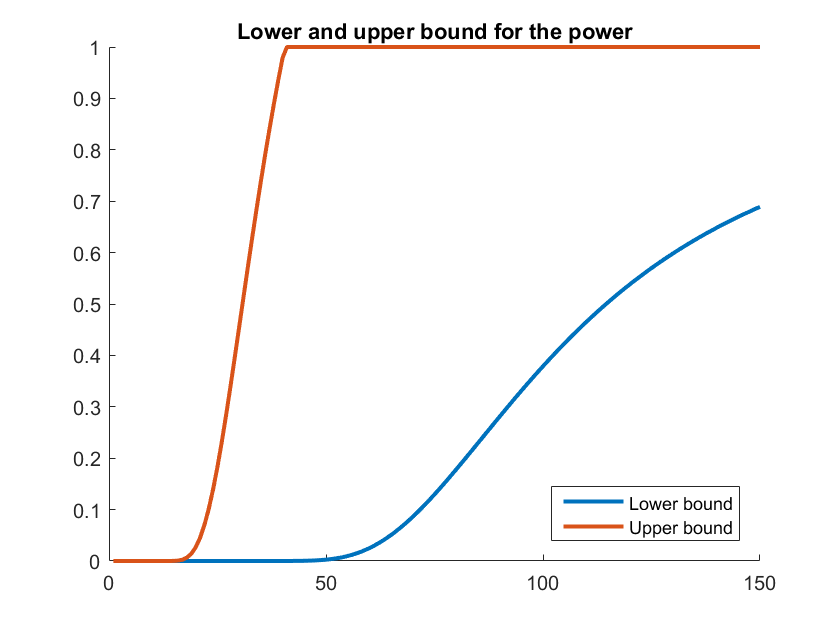
\includegraphics[width=\linewidth]{Power_Bounds}
	\caption[Power bounds]{For $\alpha = 0.05$ this graph shows the lower and upper bounds for the power of the test for $\sigma \in \{ 1, 2, \dots, 150 \}$.}
	\label{fig:demo1comparison}
\end{figure}

As we can see in the graph, we can assure, that there are no type II errors for $\sigma \in \{ 1, 2, \dots, 8 \}$. Up until $\sigma = 21$ the power stays below $\alpha = 0.05$. The upper bound increases then very fast and starting at $\sigma = 41$ we can only use the trivial upper bound, i.e. $1$. The lower bound stays at $0$ until $\sigma = 23$ and increases slowly. At $\sigma = 115$ it becomes bigger than $0.5$.

\newpage

\section{Morphological operations}

\subsection{Opening and closing}

To define opening and closing, we first need to define erosion and dilation of binary images.

\begin{definition}
	Let $A, B \subseteq \mathbb{R}^m$. The binary erosion of $A$ by $B$ is defined as
	\begin{equation*}
		A \ominus_b B = \left\{ x \in \mathbb{R}^m \mid x + b \in A \; \mathrm{for \; every} \; b \in B \right\}
	\end{equation*}
\end{definition}
\begin{definition}
	Let $A, B \subseteq \mathbb{R}^m$. The binary dilation of $A$ by $B$ is defined as
	\begin{equation*}
		A \oplus_b B = \left\{ c \in \mathbb{R}^m \mid c = a + b \; \mathrm{for \; some} \; a \in A \; \mathrm{and} \; b \in B \right\}
	\end{equation*}
\end{definition}

This can be rewritten in a more implementation-friendly form:
\begin{align*}
	(A \ominus_b B)_{(i, j)} &= \underset{m, n}{\mathrm{AND}} \left( \mathrm{OR} (A_{(i + m, j + n)}, (1 - B)_{(i, j)}) \right) \\
	(A \oplus_b B)_{(i, j)} &= \underset{m, n}{\mathrm{OR}} \left( \mathrm{AND} (A_{(i - m, j - n)}, B_{(i, j)}) \right)
\end{align*}

Where $m, n$ go through the indices, where $B = 1$. Now we can define binary opening and closing.

\begin{definition}
	The opening of an image $A$ by a structuring element $B$ is defined as
	\begin{equation*}
		A \circ B = (A \ominus B) \oplus B
	\end{equation*}
\end{definition}
\begin{definition}
	The closing of an image $A$ by a structuring element $B$ is defined as
	\begin{equation*}
		A \bullet B = (A \oplus B) \ominus B
	\end{equation*}
\end{definition}

\subsection{Hypothesis testing and opening}

From now on, we assume $B$ to be a square of ones centered around our current pixel. Using the notation from above we can take a closer look at what opening really does. We have
\begin{align*}
	(A \circ B)_{(i, j)} &= ((A \ominus B) \oplus B)_{(i, j)} \\
	&= \left( \underset{m, n}{\mathrm{AND}} \left( \mathrm{OR} (A_{(i + m, j + n)}, \underbrace{(1 - B)_{(i, j)}}_{= 0} ) \right) \right) \oplus B \\
	&= \left( \underset{m, n}{\mathrm{AND}} ( A_{(i + m, j + n)} ) \right) \oplus B \\
	&= \underset{\tilde{m}, \tilde{n}}{\mathrm{OR}} \left( \mathrm{AND} \left( \underset{m, n}{\mathrm{AND}} ( A_{(i + m - \tilde{m}, j + n - \tilde{n})} ), \underbrace{B_{(i, j)}}_{= 1} \right) \right) \\
	&= \underset{\tilde{m}, \tilde{n}}{\mathrm{OR}} \left( \underset{m, n}{\mathrm{AND}} ( A_{(i + m - \tilde{m}, j + n - \tilde{n})} ) \right)
\end{align*}

Now, we can see, that $A \circ B_{(i, j)} = 1$ if and only if $(i, j)$ is part of a square the size of $B$. In the above formula $(\tilde{m}, \tilde{n})$ determines the offset of the center of the square and thus loops through all possible positions of $(i, j)$ in the square. The inner part on the other hand assures, that there is actually a square of same size as $B$, that $(i, j)$ is part of.

We will now take a look at the effect of opening on the significance level.

\begin{theorem}
	Let $f$ be an image that contains a rectangular ROI. Assume that we are given a binarized image $f_{bin}$ with
	\begin{equation*}
		\mathbb{P}(f_{bin}(i, j) = 1 \mid H_0(i, j)) \leq \alpha
	\end{equation*}
	where $H_0(i, j)$ denotes the null hypothesis for the pixel $(i, j)$, which is, that it is a background pixel and thus should be set to zero.
	
	Let $k \in \mathbb{N}$ be odd and $B$ be a square structuring element with side length $k$. For $\tilde{m}, \tilde{n} \in \{ -\frac{k - 1}{2}, \dots, \frac{k - 1}{2} \}$ we denote by $\mathcal{G}_{(\tilde{m}, \tilde{n})}^k(i, j)$ the set of all possible ground truths in the square with side length $k$, where the pixel $(i, j)$ has offest $(\tilde{m}, \tilde{n})$ from the center of the square and assuming that the null hypothesis for the pixel $(i, j)$ is true.
	Then the following inequality holds:
	\begin{equation*}
		\mathbb{P}((f_{bin} \circ B)(i, j) = 1 \mid H_0(i, j)) \leq k^2 \alpha^k
	\end{equation*}
\end{theorem}
\begin{proof}
	First we notice that for fixed $\tilde{m}, \tilde{n}$ the set $\mathcal{G}_{(\tilde{m}, \tilde{n})}^k(i, j)$ contains ALL possible ground truths given that the null hypothesis for the pixel $(i, j)$ is true, thus
	\begin{equation*}
		\sum_{G \in \mathcal{G}_{(\tilde{m}, \tilde{n})}^k(i, j)} \mathbb{P}(G \mid H_0(i, j)) = 1
	\end{equation*}
	Second we notice, that any element $G \in \mathcal{G}_{(\tilde{m}, \tilde{n})}^k(i, j)$ already contains the null hypothesis for the pixel $(i, j)$, thus giving
	\begin{equation*}
		\mathbb{P}(G \mid H_0(i, j)) = \mathbb{P}(G)
	\end{equation*}
	Third we see that for any possible ground truth $G \in \mathcal{G}_{(\tilde{m}, \tilde{n})}^k(i, j)$ for the whole $k$ by $k$ square to be set to one in $f_{bin}$, there are at least $k$ falsely identified pixels in that square.
	
	Let $K = \{ -\frac{k - 1}{2}, \dots, \frac{k - 1}{2} \}$. Using above observations, we get
	\begin{align*}
		\mathbb{P}&((f_{bin} \circ B)(i, j) = 1 \mid H_0(i, j)) \\
		&= \mathbb{P} \left( \bigcup_{\tilde{m}, \tilde{n} \in K} \bigcap_{m, n \in K} ( f_{bin}(i + m - \tilde{m}, j + n - \tilde{n}) = 1 ) \mid H_0(i, j) \right) \\
		&= \sum_{\tilde{m}, \tilde{n} \in K} \mathbb{P} \left( \bigcap_{m, n \in K} ( f_{bin}(i + m - \tilde{m}, j + n - \tilde{n}) = 1 ) \mid H_0(i, j) \right) \\
		&= \sum_{\tilde{m}, \tilde{n} \in K} \sum_{G \in \mathcal{G}_{(\tilde{m}, \tilde{n})}^k(i, j)} \mathbb{P}(G \mid H_0(i, j)) \cdot \mathbb{P} \left( \bigcap_{m, n \in K} ( f_{bin}(i + m - \tilde{m}, j + n - \tilde{n}) = 1 ) \mid G, H_0(i, j) \right) \\
		&= \sum_{\tilde{m}, \tilde{n} \in K} \sum_{G \in \mathcal{G}_{(\tilde{m}, \tilde{n})}^k(i, j)} \mathbb{P}(G) \cdot \underbrace{\mathbb{P} \left( \bigcap_{m, n \in K} ( f_{bin}(i + m - \tilde{m}, j + n - \tilde{n}) = 1 ) \mid G, H_0(i, j) \right)}_{\leq \alpha^k} \\
		&\leq \sum_{\tilde{m}, \tilde{n} \in K} \sum_{G \in \mathcal{G}_{(\tilde{m}, \tilde{n})}^k(i, j)} \mathbb{P}(G) \cdot \alpha^k \\
		&= \alpha^k \cdot \sum_{\tilde{m}, \tilde{n} \in K} \underbrace{\sum_{G \in \mathcal{G}_{(\tilde{m}, \tilde{n})}^k(i, j)} \mathbb{P}(G)}_{= 1} = \alpha^k \cdot \sum_{\tilde{m}, \tilde{n} \in K} 1 = \alpha^k \cdot \abs{K}^2 = k^2 \alpha^k
	\end{align*}
\end{proof}

\subsection{Hypothesis testing and closing}
In a similar way as above, we can also see, what closing does. We have
\begin{align*}
	(A \bullet B)_{(i, j)} &= ((A \oplus B) \ominus B)_{(i, j)} \\
	&= \left( \underset{m, n}{\mathrm{OR}} \left( \mathrm{AND} (A_{(i - m, j - n)}, \underbrace{B_{(i, j)}}_{= 1} ) \right) \right) \ominus B \\
	&= \left( \underset{m, n}{\mathrm{OR}} ( A_{(i - m, j - n)} ) \right) \ominus B \\
	&= \underset{\tilde{m}, \tilde{n}}{\mathrm{AND}} \left( \mathrm{OR} \left( \underset{m, n}{\mathrm{OR}} ( A_{(i - m + \tilde{m}, j - n + \tilde{n})} ), \underbrace{(1 - B)_{(i, j)}}_{= 0} \right) \right) \\
	&= \underset{\tilde{m}, \tilde{n}}{\mathrm{AND}} \left( \underset{m, n}{\mathrm{OR}} ( A_{(i - m + \tilde{m}, j - n + \tilde{n})} ) \right)
\end{align*}

\subsection{Convex hull}

As we have seen in the section about multiple testing procedures, we defined the family-wise error rate as $\mathbb{P}(V \geq 1) = 1 - \mathbb{P}(V = 0)$.

\newpage

\section{Multiple testing procedures}

In a next step, we want to employ one of three multiple testing procedures. Consider the following setup:
\begin{table}[h]
	\tymax .3\textwidth
	\begin{tabulary}{\textwidth}{|CCCC|}
		\hline
		& \textit{Declared non-significant} & \textit{Declared significant} & \textit{Total} \\
		\hline
		\textit{True null hypotheses} & $\mathbf{U}$ & $\mathbf{V}$ & $m_0$ \\
		\textit{Non-true null hypotheses} & $\mathbf{T}$ & $\mathbf{S}$ & $m - m_0$ \\
		& $m - \mathbf{R}$ & $\mathbf{R}$ & $m$ \\
		\hline
	\end{tabulary}
\end{table}

\begin{itemize}
	\item $m$ is the total number hypotheses tested
	\item $m_0$ is the number of true null hypotheses, an unknown parameter
	\item $m - m_0$ is the number of true alternative hypotheses
	\item $V$ is the number of false positives (Type I error) (also called "false discoveries")
	\item $S$ is the number of true positives
	\item $T$ is the number of false negatives (Type II error)
	\item $U$ is the number of true negatives
	\item $R = V + S$ is the number of rejected null hypotheses (also called "discoveries", either true or false)
\end{itemize}
In $m$ hypothesis tests of which $m_0$ are true null hypotheses, $R$ is an observable random variable, and $S$, $T$, $U$, and $V$ are unobservable random variables.

We define another random variable $Q = \frac{V}{V + S}$, which is the proportion of the rejected null hypotheses which are erroneously rejected. We set $Q = 0$, if $V + S = 0$. Based on this, we define the false discovery rate to be
\begin{equation}
	FDR = \mathbb{E}(Q) = \mathbb{E} \left( \frac{V}{V + S} \right)
\end{equation}

We also define the family-wise error rate to be
\begin{equation}
	FWER = \mathbb{P}( V \geq 1 ) = 1 - \mathbb{P}( V = 0 )
\end{equation}
that is the probability of making one or more type I errors.

Three of these multiple testing procedures are given in detail in the following. The first one controls the false discovery rate at level $\alpha$, i.e.
\begin{equation}
	FDR = \mathbb{E}(Q) \leq \alpha
\end{equation}

The other two procedures control the family-wise error rate at level $\alpha$, i.e.
\begin{equation}
	FWER = \mathbb{P}( V \geq 1 ) \leq \alpha
\end{equation}

First, we calculate for every pixel $(i, j) \in G$ the $p$-value
\begin{equation}
	p(i, j) = \exp \left( - \frac{\tilde{d}(i, j)^2}{4 \sigma^2} \right) \geq \mathbb{P}(T \geq \tilde{d}(i, j) \mid H_0)
\end{equation}

\subsection{FDR Thresholding}
\begin{enumerate}[(i)]
	\item Sort $p$-values in ascending order: $p_{(1)} \leq p_{(2)} \leq \dots \leq p_{(M \cdot N)}$
	\item Calculate the maximal index $k$, such that $p_{(k)} \leq \frac{k \cdot \alpha}{M \cdot N}$
	\item Calculate the threshold $\lambda_{k} = 2 \sigma \sqrt{- \log(p_{(k)})}$
	\item Reject all hypotheses $H_{(i)}$ with $p_{(i)} \leq p_{(k)}$, i.e. all hypotheses with $$\tilde{d}_{(i)} \geq \tilde{d}_{(k)} = \lambda_{k} = 2 \sigma \sqrt{- \log(p_{(k)})}$$
\end{enumerate}

\subsection{Bonferroni Thresholding}
\begin{enumerate}[(i)]
	\item Reject all hypotheses $H_{i}$ with $p_{i} \leq \frac{\alpha}{M \cdot N}$, i.e. all hypotheses with $$\tilde{d}_{i} \geq \lambda_k = 2 \sigma \sqrt{- \log \left( \frac{\alpha}{M \cdot N} \right)}$$
\end{enumerate}

\subsection{Hochberg Thresholding}
\begin{enumerate}[(i)]
	\item Sort $p$-values in ascending order: $p_{(1)} \leq p_{(2)} \leq \dots \leq p_{(M \cdot N)}$
	\item Calculate the maximal index $k$, such that $p_{(k)} \leq \frac{\alpha}{M \cdot N - k + 1}$
	\item Reject all hypotheses $H_{(i)}$ with $p_{(i)} \leq p_{(k)}$, i.e. all hypotheses with $$\tilde{d}_{(i)} \geq \tilde{d}_{(k)} = \lambda_{k} = 2 \sigma \sqrt{- \log(p_{(k)})}$$
\end{enumerate}

\begin{remark}
	All these methods are defined for actual $p$-values, i.e.
	\begin{equation*}
		p(i, j) = \mathbb{P}(T \geq \tilde{d}(i, j) \mid H_0)
	\end{equation*}
	In contrast to that, we have taken upper bounds for the $p$-values. This is not an issue though, since by taking upper bounds we might decrease the number of hypotheses we reject. Thus it will not increase the error rate.
\end{remark}

\begin{remark}
	The threshold has the following interpretation:
	\begin{itemize}
		\item If $\tilde{d}(i, j) \geq \lambda_{k}$, then $(i, j)$ is part of the ROI.
		\item If $\tilde{d}(i, j) < \lambda_{k}$, then $(i, j)$ is NOT part of the ROI.
	\end{itemize}
\end{remark}

\newpage

\subsection{Example}
\begin{figure}[h]
	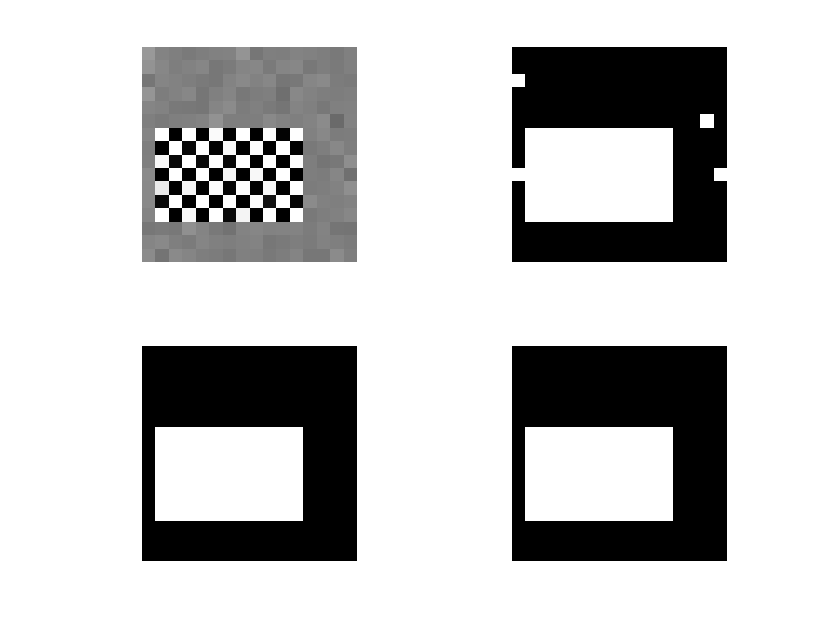
\includegraphics[width=\linewidth]{Thresholding_Comparison}
	\caption[Comparison of different thresholding procedures]{The top left is the original image f of testDemo.mat, top right is the ROI with FDR thresholding, bottom left is the ROI with Bonferroni thresholding and bottom right is the ROI with Hochberg thresholding. (Standard deviation of the noise is $\sigma = 7$.)}
	\label{fig:demo1comparison}
\end{figure}
	
\end{document}